\begin{center}
\scriptsize
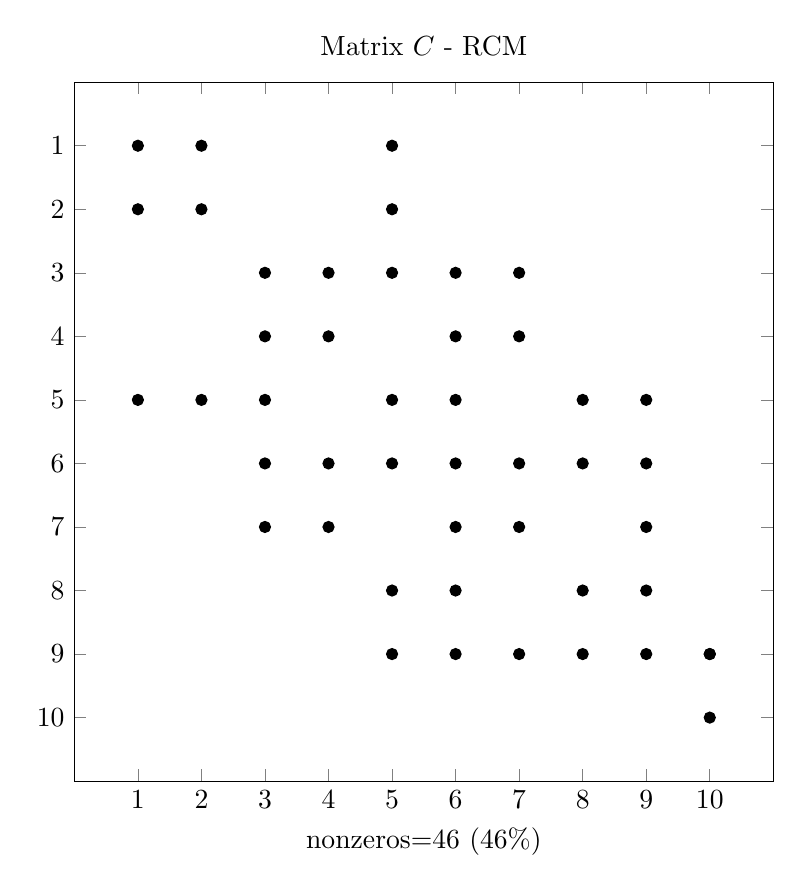
\begin{tikzpicture}
    [   baseline = {(current bounding box.north)}
    ]
    \begin{axis}
        [   unit vector ratio* = 1 1 1
        ,   y dir = reverse
        ,   xmin = 0
        ,   ymin = 0
        ,   xmax = 11
        ,   ymax = 11
        ,   title = {Matrix $C$ - RCM}
        ,   xlabel = {nonzeros=46 (46\%)}
        ,   width = \linewidth
        ,   xtick = {1,2,3,4,5,6,7,8,9,10}
        ,   ytick = {1,2,3,4,5,6,7,8,9,10}
        ]
        \addplot[only marks] coordinates
        {   (1,1)(2,1)          (5,1)
            (1,2)(2,2)          (5,2)
                      (3,3)(4,3)(5,3)(6,3)(7,3)
                      (3,4)(4,4)     (6,4)(7,4)
            (1,5)(2,5)(3,5)     (5,5)(6,5)     (8,5)(9,5)
                      (3,6)(4,6)(5,6)(6,6)(7,6)(8,6)(9,6)
                      (3,7)(4,7)     (6,7)(7,7)     (9,7)
                                (5,8)(6,8)     (8,8)(9,8)
                                (5,9)(6,9)(7,9)(8,9)(9,9)(10,9)
                                                   (10,9)(10,10)
        };
    \end{axis}
\end{tikzpicture}
\end{center}
